\documentclass[compress]{beamer}
\usetheme{default}
\usecolortheme{default}
\usepackage{amsbsy,amsmath,latexsym,amsfonts,subfigure,enumerate}
\usepackage{hyperref}
\usepackage{makecourse}
\usepackage{graphicx}
\setbeamertemplate{navigation symbols}{}
\title{Sample Slides}
\author{Ann Example}
\institute{}
\date{}
\setbeamertemplate{blocks}[framed]

\begin{document}

\begin{frame}[t]
	\frametitle{Series Results}
	\begin{eqnarray*}
		\sum_{x=0}^{\infty} q^x &=& \frac{1}{1-q}, \ |q|<1. \\
		\frac{d}{dx}\left(\sum_{x=0}^{\infty} q^x \right) &=& \sum_{x=0}^{\infty} xq^{x-1}=\sum_{x=1}^{\infty} xq^{x-1} = \frac{1}{(1-q)^2}, \ |q|<1. \\
		\sum_{x=0}^{N} q^x &=& \frac{1-q^{N+1}}{1-q}. \\
		\sum_{n=0}^{\infty} \frac{x^n}{n!} &=& 1+x+\frac{x^2}{2!}+\frac{x^3}{3!}+\ldots = e^x
	\end{eqnarray*}
\end{frame}

\begin{frame}[t]
\frametitle{Expectation}
{\bf Discrete Random Variables}
\begin{eqnarray*}
E[g(X)] &=& \sum_{x \in S} g(x) Pr(X=x) \\
Var(X)  &=& E[X^2] - E[X]^2.
\end{eqnarray*}
{\bf Continuous Random Variables}
\begin{eqnarray*}
E[g(X)] &=&  \int_{-\infty}^{\infty} g(x) f_X(x) dx \\
Var(X)  &=& E[X^2]-E[X]^2.
\end{eqnarray*}
\end{frame}

\begin{frame}[t]
\frametitle{Families of Discrete Random Variables I}
{\bf Bernoulli random variables, $X \sim Bern(p)$}
\begin{eqnarray*}
Pr(X=x) &=& \left\{ \begin{array}{cc} p, & x=1, \\ 1-p, & x=0. \end{array} \right.
\end{eqnarray*}
\[
E[X] = p \qquad Var(X) = p(1-p).
\]
{\bf Binomial random variables, $X \sim Bin(n,p)$} 
\begin{eqnarray*}
Pr(X=x) &=& \left( \begin{array}{c} n \\ x
      \end{array} \right) p^x (1-p)^{n-x},\  x=0,1,\ldots,n,
\end{eqnarray*}
\[
E[X] = np \qquad Var(X) = np(1-p).
\]
{\bf Poisson random variables, $X \sim Po(\lambda), \ \lambda>0$}
\begin{eqnarray*}
Pr(X=x) &=& \frac{\lambda^x e^{-\lambda}}{x!}, \ x=0,1,2,\ldots.
\end{eqnarray*}
\[
E[X] = \lambda \qquad Var(X) = \lambda.
\]
\end{frame}

\begin{frame}[t]
\frametitle{Families of Discrete Random Variables II}

{\bf Geometric random variables, $X \sim Geom(p)$}
\begin{eqnarray*}
Pr(X=x) &=& p(1-p)^{x-1}, \ x=1,2,\ldots.
\end{eqnarray*}
\[
E[X] = \frac{1}{p} \qquad Var(X) = \frac{1-p}{p^2}.
\]
{\bf Negative Binomial random variables, $X \sim NBin(r,p)$} 
\begin{eqnarray*}
Pr(X=x) &=& \left( \begin{array}{cc} x-1 \\ r-1 \end{array} \right) p^r (1-p)^{n-r}, \ x=r,r+1,\ldots.
\end{eqnarray*}
\[
E[X] = \frac{r}{p} \qquad Var(X) = \frac{r(1-p)}{p^2}. 
\]
{\bf Discrete Uniform random variables, $X \sim U(1,2,\ldots,n)$}
\begin{eqnarray*}
Pr(X=x) &=& \frac{1}{n}, \ x=1,2,\ldots,n.
\end{eqnarray*}
\[
E[X] = (n+1)/2 \qquad Var(X) = (n^2-1)/12.
\]
\end{frame}


\begin{frame}[t]
\frametitle{Families of Continuous Random Variables I}

{\bf Uniform random variables}, $X \sim U(a,b)$,
\begin{eqnarray*}
f_X(x) &=& \frac{1}{b-a}, \ a < x < b.
\end{eqnarray*}
\[
E[X]=\frac{a+b}{2} \qquad Var(X) = \frac{(b-a)^2}{12}.
\]
{\bf Exponential random variables}, $X \sim Exp(\lambda)$, 
\begin{eqnarray*}
f_X(x)&=& \lambda e^{-\lambda x}, \ x>0, \ \lambda>0.
\end{eqnarray*}
\[
E[X]= \frac{1}{\lambda} \qquad Var(X) = \frac{1}{\lambda^2}.
\]
{\bf Normal random variables}, $X \sim N(\mu,\sigma^2)$, 
\[
f_X(x) = \frac{1}{\sqrt{2\pi \sigma^2}} e^{-\frac{(x-\mu)^2}{2\sigma^2}}, \ -\infty < x < \infty, \ -\infty < \mu < \infty, \ \sigma>0.
\]
\[
E[X]= \mu \qquad Var(X) = \sigma^2.
\]
\end{frame}

\begin{frame}[t]
\frametitle{Families of Continuous Random Variables II}
{\bf Gamma random variables}, $X \sim Ga(n,\lambda)$,
\[
f_X(x) = \frac{\lambda^{n}}{\Gamma(n)} x^{n-1}
e^{-\lambda x}, \qquad x>0, \ n>0,\ \lambda>0, \ \Gamma(n)=(n-1)!
\]
\[
E[X] = \frac{n}{\lambda} \qquad Var(X) = \frac{n}{\lambda^2}. 
\]
{\bf Beta random variables}, $X \sim Beta(a,b)$,
\begin{eqnarray*}
f_X(x) &=& \frac{1}{B(a,b)} x^{a-1}(1-x)^{b-1} \\
&=&  \frac{\Gamma(a+b)}{\Gamma(a)\Gamma(b)} x^{a-1}(1-x)^{b-1},\qquad 0<x<1, \ a>0, \ b >0. 
\end{eqnarray*}
\[
E[X]=\frac{a}{a+b} \qquad  Var(X) = \frac{ab}{(a+b)^2(a+b+1)}.
\]
\end{frame}

\begin{frame}
\frametitle{Column example}
\begin{columns}
\begin{column}{0.6\textwidth}
   Here is some text in a left hand column.
\end{column}
\begin{column}{0.4\textwidth}
     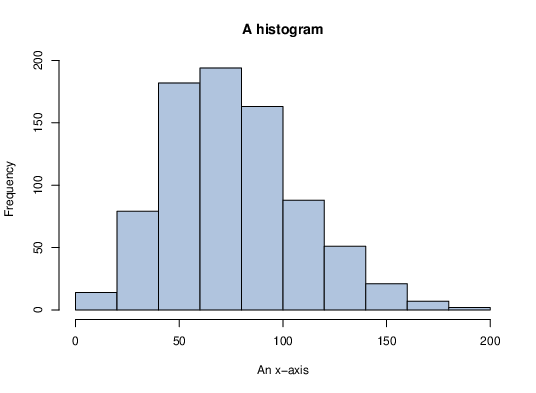
\includegraphics[width=\textwidth]{image.png}
	 \alttext{An image showing an example plot of a histogram.}
\end{column}
\end{columns}
\end{frame}

\end{document}
